\label{chap:political_sides}

\section{\statusorange Introduction}

% In this chapter we investigated the persuasion techniques. But we have not studied the relationship between this observed persuasion in the text and the ideals/agenda/perspective of the author/outlet. It can be really useful to understand the context around the source of an article in order to interpret its persuasion.
% For this reason, the next chapter will consider perspectives and political sides. In this way we will try to understand if the persuasion of each political side is similar or which are the differences. If a different goal for the persuasion also can be observed on the persuasion itself.

In this new chapter, we introduce a new factor in our analysis.
Having in the previous one covered persuasion and propaganda, we demonstrated the need to understand the context around the source of an article in order to interpret its persuasion means.

For this reason, this chapter introduces the factor of \emph{perspectives and political sides}.
Our goal is to see and understand how persuasion (and more specifically propaganda) varies across the political spectrum. If political points of view of the sources can be so diverse, what are the techniques that they use differently in news articles to persuade the readers? Is there a link between the political orientation and the persuasion used?
% How does political point of view influence the usage of propaganda?

% Perspectives and Political Sides. What drives  the variations and propaganda? Which political interests? 

Our Research Questions for this chapter are:
\begin{itemize}
    \item How does propaganda vary across the political spectrum?
    \item Can we predict the political leaning of a news article by observing the propaganda it uses?
    \item Is Propaganda Detection balanced? Or is there some imbalance in the datasets used in the literature?
\end{itemize}

\todo{list contributions of this chapter}

For this chapter, we follow the structure from the previous one~\ref{chap:linguistic_persuasion}:
\begin{itemize}
    \item first, in Section~\ref{sec:ps_political_sides}, we introduce the new ingredient: political leaning. We describe the datasets in use and the task of political leaning prediction;
    \item then, in Section~\ref{sec:ps_prop_and_leaning}, we combine the analysis of political leaning with the analysis of the previous chapters. More in specific, we analyse the relationship between propaganda and political leaning.
\end{itemize}


\section{\statusred Political Leaning Prediction}
\label{sec:ps_political_sides}

Here we describe Political Leaning Prediction.

As we already described in the literature chapter~\ref{sec:lit_leaning}, 

\subsection{Political Leaning Definition}

From literature

Political leaning over Left/Right axis: Left/Right definitions

Points from Left and Right ideologies (inspired by AllSides and Wikipedia and cite others) 

Disclaimer US vs the rest?

Several axes when describing news sources: L/R, factuality, 

\subsection{Datasets for Political Leaning Prediction}

Datasets annotating sources:

- MBFC
- AllSides

Datasets of articles? Is article always considered with the same leaning as source?

\subsection{Models for Political Leaning Prediction}

How it is computed

Usual features

State of the Art

Problems: learning the source instead of learning L/R task

\subsection{Our datasets and experiments of prediction}

\section{\statusorange Propaganda and Political Leaning Prediction}
\label{sec:ps_prop_and_leaning}

Here we want to see the relationship between Propaganda (studied in the previous Chapter~\ref{ssec:lp_techniques_propaganda} and Political Leaning (from the previous Section~\ref{sec:ps_political_sides}.

\subsection{\statusorange Propaganda across political spectrum}
% From Experiment 4.3: comparison of sentiment/propaganda across political leaning

Our first RQ for this chapter is: \emph{How does propaganda vary across the political spectrum?}

Instead of measuring the effect of removing the “framing” pieces on clustering algorithms, here we want to observe what is the effect on document similarity between different sources.
Given articles from the left/center/right, we want to compare if there is a change in similarity when we remove sentiment and propaganda terms (e.g., articles are more similar than before).
Hypothesis
When removing propaganda/sentiment some political sides will be more similar to others. This is because the different parts are related to the propaganda/sentiment which is an added layer on top of the facts described.

1. Extraction of propaganda/sentiment
Each article is analysed independently from the others, using the propaganda detection method and the sentiment lexicons.
The percentages of words annotated with respect to the total number of words are computed for each article.
2. Grouping the percentages by political bias
Considering the labels given by AllSides (left, lean-left, center, lean-right, right, mixed, not-rated), the average of sentiment-words-ratio, propaganda-words-ratio and both-ratio are computed. This gives an idea of how much of the articles from each political side is detected as sentiment-related or propaganda-related.

\begin{figure}[!htbp]
    \centering
    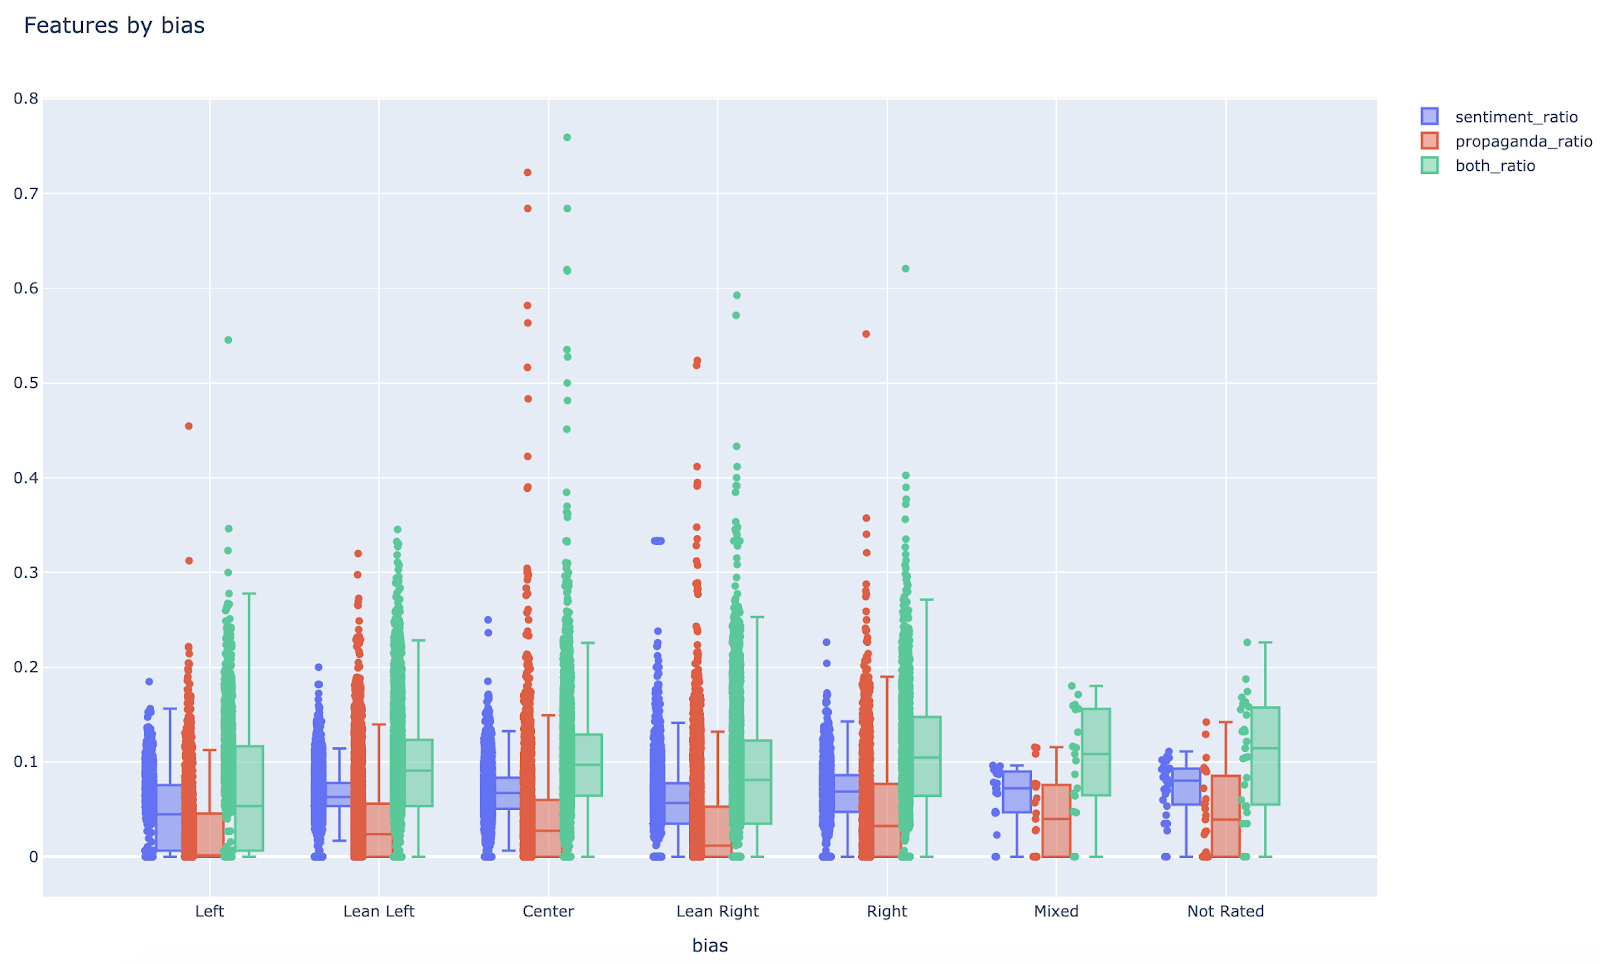
\includegraphics[width=\linewidth]{figures/4.3_prop_sent_across_leaning.png}
    \caption{Caption}
    \label{fig:prop_sent_across_leaning}
\end{figure}
\todo{Replace Figure~\ref{fig:prop_sent_across_leaning} with the one cleaned down in google docs}

This plot in Figure~\ref{fig:prop_sent_across_leaning} is a quartile representation (with data points on the left of the boxes) which shows the distribution of the ratios computed. We can see that the average value (the line in the middle of the box) of “both\_ratio” is the highest for the “Right” side.
From this plot we see that there are some very strange values (76\% of highlighted words in one article from the center). Looking at the details, this is an article from BBC which does not look so subjective. The problem is that from the full article, the scraping library only captured the sentence The statement says: "It is an assault on UK sovereignty and any such use by a State party is a clear violation of the Chemical Weapons Convention and a breach of international law. It threatens the security of us all." which is annotated as almost everything propaganda. For other BBC articles, scraping manages to retrieve the full text without problems.

There are also a lot of articles which have a percentage of 0\%. Looking at the distribution of the length of the documents, some documents, especially from some sources, have length=0 or a very short length (scraping the cookie disclaimer instead of the full article).
For this reason a minimum length threshold has been set to cut out these problems: 150 tokens at least.

This is the same plot, but with the filter on the minimum length.
We can see that:
The most annotated side is the Right
The least annotated side is the Left
Article from the Center do not contain less sentiment/propaganda (against assumption)
There are less propaganda words than sentiment words



3. Creation of modified documents without the sentiment/propaganda parts
As in the previous experiment (clustering), for each document other three documents have been created:
Without propaganda words
Without sentiment words
Without propaganda and sentiment words
Each document is embedded with two different methods:
Universal Sentence Encoder
TF-IDF (TODO dimensionality reduction, now it is a local TF-IDF to the cluster, see next point)


4. Comparing the articles about the same story
Using the labels from AllSides, where articles are put together in groups of three items (usually one from the left, one from the center, one from the right), we compute the pairwise similarity matrix by using the embedded representations.
For each cluster (provided by AllSides) we have 12 documents:
Left-Full: the article from the left side, the full text
Left-NoSent: the article from the left side, without sentiment words
Left-NoProp: the article from the left side, without propaganda words
Left-NoBoth: the article from the left side, without propaganda and sentiment words
Center-Full: the article from the center side, the full text
Center-NoSent: the article from the center side, without sentiment words
Center-NoProp: the article from the center side, without propaganda words
Center-NoBoth: the article from the center side, without propaganda and sentiment words
Right-Full: the article from the right side, the full text
Right-NoSent: the article from the right side, without sentiment words
Right-NoProp: the article from the right side, without propaganda words
Right-NoBoth: the article from the right side, without propaganda and sentiment words
These articles are compared with a 12x12 matrix where the values are the similarity between the pair of docs.
NOTE: at the moment, TF-IDF is computed locally to each cluster. I need to do the dimensionality reduction to be able to scale to more documents

These similarities are then merged for all the AllSides clusters (being careful with the labels which can be different) and a final matrix is computed by doing an average of the matrices from the single clusters.
The result is a 24x24 matrix (6 bias labels, not only left/center/right, multiplied with 4 variations of the same article).
With this matrix it is possible to observe if, removing some parts of the articles, the similarity scores increase or decrease between different political sides.


Results

\todo{figures import}

Observations:
Within the rectangles on the main diagonal (yellow bright): comparison of the original articles with the modified ones generated from it:
The removals are not changing the representations a lot: the scores are all quite high (minimum around 92% of similarity)
The removal of propaganda parts is keeping the documents very similar to the original ones: average 98% similarity
The removal of sentiment is changing a bit more the representation of the articles: minimum 93%, average 95%
Increasing values between different biases (main diagonal of each block, see below):
Usually similarity increases from Full article to noBoth
Removing sentiment increases similarity (best scores)
Removing propaganda decreases similarity a bit
TODO: find a better way to represent this result. Just look at the main diagonals of each block, not so interesting to see the comparison between full articles and 

Further improvements (TODOs):
Propaganda/sentiment used by political sides by topic: break down by topic
Propaganda types and sentiment scores by political sides: break down by fine-grained labels
Verify correlation between propaganda:loaded\_language and sentiment. It is probably the same thing
Improve visualisations of similarity changes (heatmap so big is confusing)
Use dimensionality reduction and use a single TF-IDF model

\todo{the rest goes in topic breakdown (next chapter)}


Types of shapes (propaganda)
(look at purple: propaganda)

Blue is sentiment (+ and -) and purple is propaganda. 
y axis in the fraction of terms marked as sentiment/propaganda.




\subsection{\statusorange Political leaning prediction using propaganda features}

% 5: political leaning classifier from propaganda features. Why


RQ2: \emph{Can we predict the political leaning of a news article by observing the propaganda it uses?}

Why the two could benefit / be related?

The point of contact between political leaning prediction and propaganda is that both are dealing with political analysis.
Given that the facts that are being narrated are the same (exception: inclusion/exclusion), the main difference between an article from the left to one from the right is their point of view / subjective / persuasive component. Propaganda analysis is focused on analysing this specific component of the articles, the anti-topic model.
On this, we have our hypothesis that \emph{we can recognise the political leaning of an article by using the features provided by the propaganda analysis}.
The mixed analysis would allow to understand better why a certain article is classified as being left/right with respect to the black box BERT classifier.

The following sections first describe the general setup of the experiment, then deal with each one of the three research questions that we listed in the introduction: quantity, quantity by type, terms analysis.% TODO , context.


Unlike previous work on political leaning detection, in this paper we use a propaganda detection method (from \citet{da2019fine}) to identify the existence of propaganda and its type of technique in given articles, and incorporate this information directly as additional features into the training and testing of the model.  

\todo{copy from experiment 4.3 / TTO paper}

% THIS IS FROM CIMPLE REPORT / TTO paper
Understanding the implicit political leaning of news articles could be seen as an indicative factor for identifying misinformation [13]. In the experiment reported in this section, different types of propaganda used in news articles are used for identifying the political leaning of the articles. 
Propaganda is a regularly used technique in media and politics that aims to influence the perception of the audience and to sway their opinions in specific directions. However, it is unclear to what extent can we automatically identify the political leaning of news from their use of propaganda. This experiment investigates the use of propaganda features as input to an automated political leaning classifier.
Propaganda is usually directly linked to the ideology of articles by having the “intention of influencing people’s opinions”. To this end, we aim to better understand the relationship between propaganda analysis and the identification of political leaning of articles, simplified to three categories: Left, Centre, and Right.
Our hypothesis is that it is possible to recognise the political leaning of an article by using the features extracted through propaganda analysis. In other words, we hope to boost the performance of political leaning classifiers by learning which and how propaganda techniques are being used by which political side. This leads to three research questions (RQ), aimed to see if it is possible to recognise the political leaning of articles from the:
Total amount of propaganda found in the text (RQ1)
Amount of each propaganda technique in the text (RQ2)
Specific words belonging to propaganda techniques in the article text (RQ3)
In this experiment, we use a propaganda detection method proposed in [14] to identify the existence of propaganda and its type of technique in given articles, and incorporate this information directly as additional features into the training and testing of the model.

\subsubsection{Dataset}
The dataset used in this experiment [15] consists of articles in English language from over 800 sources (majority from the US), labelled for their political leaning (Left, Centre or Right). This dataset contains several attributes for each article: full text, political leaning, topic, news source, and author name. However, in our models and experiments, we only use the text of the articles to avoid bias associated with the other attributes. The topic distribution of the articles is uniform across the political leanings, because the dataset comes from triples of articles, one from each political leaning, about the same issue. The dataset contains two pre-split folds for training and testing:
Random: where splits are randomly generated. This classification model might encounter articles from the same media source during both training and testing phases.
Media: where the articles in the test set are from media sources that do not occur in the training set.

\subsubsection{Experimental Setup}

The following steps are followed in this experiment:
 Implement the BERT-based political-leaning classifier described in [15] and apply it to the dataset to detect the political leaning of each article to reproduce the baseline results.
 Extract propaganda for each article using the tool from [14].
Add propaganda-related features to the BERT model, by injecting the values in the neural network using the (a) total presence of propaganda as a feature (Experiment 1), (b) percentage of each propaganda technique (Experiment 2), and (c) words that appear in the detected propaganda text (Experiment 3).
Train and test the model under different configurations with two splits, one   one less biased to media source.
Compare our results with two baselines; the majority class (where the political leaning is assumed to be that of the most popular leaning in the dataset), and the results from our re-implementation of the model in step 1

\paragraph{Political Leaning Model}
Our baseline for article-level political leaning is [15], which is the current state of the art for general purpose political leaning classification. Since the source code for this work is yet to be released, we reproduced the architecture of the model by following the details provided by the authors. Note, however, that the results we reproduced differ from those reported in their paper. This could be because of possible slight reimplementation discrepancies, and of the difference between the dataset reported in their paper and the one they shared on GitHub. Table 6 shows the results we reproduced, which form our baseline (Baly-baseline).
We embed the articles in our dataset with a pre-trained BERT model (110M parameters, uncased5) and use the vectors from the second-to-last layer, as in [15].

\todo{table}

\paragraph{Propaganda Features}
The extraction tool [14] extracts 18 propaganda techniques (listed in Figure 5). We apply this tool to the articles in our dataset to obtain these propaganda annotations. We use these annotations to calculate several numerical features that we employ in the following three sections to answer the three research questions.
Our analysis workflow is depicted in Figure 6. Each article in the dataset is passed through the baseline BERT pre-trained models to calculate the baseline result, and through our models that incorporate the various propaganda features to calculate the results from our three experiments.
We calculate the F1-macro and accuracy of the models and compare them with each other and with the baseline. We also evaluate the significance of each added feature from the weight assigned to them by the classification model (the higher the weight, the more discriminative the feature is for Left/Centre/Right-leaning articles). We also combine the features given by each feature set, to see whether the addition of certain features helps to achieve higher classification accuracy. This combination is performed by concatenating the inputs to the SoftMax dense layer. It is not a combination of trained models, but it is a model that is trained and used on a combination of input features.

\todo{figure}

\subsubsection{Total Quantity of Propaganda}
Considering only the total amount of propaganda in each article, we calculate a single value to represent the percentage of propaganda text inside the article (i.e., the ratio between the number of propagandist words and the total number of words) to answer RQ1.
Figure 7 shows how this value is distributed across Left, Centre and Right leaning articles. Table 6 shows the results of this first experiment under the name Prop-Total. The low values, just above the Majority baseline, indicate that the feature is unsuitable for determining which side an article belongs to. Both F1 and accuracy are below the values of Baly-baseline for both Random and Media splits. Thus, the answer to RQ1 is No, the total amount of propaganda in an article does not seem to be a good indicator of the political leaning of an article.

\subsubsection{Quantity of Propaganda Techniques}
Testing the role of the presence of particular propaganda techniques in determining the political-leaning, RQ2, compute the word-based percentage of each technique inside each article and used the features obtained to classify articles. The value for each technique is equal to the number of words belonging to it, divided by the total number of words in the document.
We train the classifiers as the in previous experiment and obtain the result indicated by Prop-Techniques (2) in Table 6. Although the results show improvement over the previous experiment, they are still well below the best performing baseline. The results show that (a) Prop-Techniques alone is insufficient to accurately detect the political leaning of articles (RQ2), and (b) when Prop-Techniques is added to Baly-baseline (line (0) + (2) in results table), it brings an improvement on the Media split for both the F1 and accuracy measures. 
Given the improvements in some cases, we perform an additional test to better understand the significance of these results. To perform this test, we build a contingency table by considering two arrays: the first shows when the Baly-baseline produced the correct result on the test set, and the second one shows when the line (0) + (2) (baseline+propaganda techniques quantity) produced the correct result on the Media split. The contingency table, therefore, is a 2x2 matrix.
Using the predicted labels of the selected rows on the Media split (last two columns of Table 6), the (0)+(2) against baseline resulted in a pvalue=0:008, which means that the improvement is significant. Remember that the Media split is less biased than the Random split, since in the Media split the sources of the articles in the test set are not overlapping with the sources of the articles in the training set. If we compare the Random vs Media split results, we can see that while the Baly-baseline drops significantly (more than 15\% F1 and 12\% accuracy), the models based on the features of propaganda have a much smaller drop in these measures (less than 8\% F1 and less than 1\% accuracy). This means that our models with propaganda features are coping better with articles from “new sources” that are unseen in the training set. The improved generalisation abilities of this feature are perhaps what is driving the significant improvement described above.
The conclusion of this experiment is that the amount of each propaganda technique is not enough on its own to accurately recognise the political leaning of an article, but when combined with the baseline features produces a significant improvement.


\subsubsection{Terms of Propaganda}

To investigate the chosen terminology for expressing the identified propaganda techniques in articles for each political leaning (RQ3), the terms were analysed in two different ways:
(3a) all the propaganda words taken together: non-propaganda annotated words are filtered out. The classifier will then use the remaining propaganda words to learn any differences between political leanings.
(3b) propaganda words grouped by propaganda technique: there are 18 groups, one for each propaganda technique. The classifier will use the words, grouped by the technique to which they belong, to recognise the political leaning.
To obtain the feature vectors of the propaganda words, we use TF-IDF because its numerical values directly represent single terms. Instead with other embedding methods  this correspondence with single terms would be more difficult to extract. By considering the features which get assigned the biggest values in the final SoftMax layer, we can directly say which terms are the most discriminative for the task of political leaning classification. 
The row of Table 6with the label Prop-Total-Terms (3a) refers to the TF-IDF features computed by only using the propaganda terms, without differentiating between the different techniques. This row has significantly better results than (1) and (2) on both splits, but only outperform the Baly-baseline on the Media split in F1.
On the other hand, the feature Prop-Techniques-Terms (3b) refers to splitting the propaganda terms into the 18 groups and then computing the TF-IDF features on each group separately. The results of this feature set are generally a few decimal points below (3a).
With the current analysis, we can say that the answer to RQ3 is a partial Yes: using as feature the terms of propaganda achieves a very similar score to the baseline (rows indicated with (3a) and (3b)), and when added to the baseline features, it helps to achieve a small (but not significant, p-value=0.657) improvement.


\subsubsection{Conclusion}

This experiment analysed the relationship between propaganda and political leaning detection as the political leaning is an indicative factor for detecting misinformation in political context [13]. Using available works for propaganda detection and political leaning, we explored the effects of the propaganda features on the task of political leaning prediction. We showed that (a) propaganda is equally found in Left, Centre, and Right leaning articles, (b) detecting political leanings with propaganda features is challenging, and (c) detection performance improves when we use the amount of each propaganda technique together with the baseline features (0)+(2). The appearance of propaganda, and the techniques used, showed not to be sufficient by themselves in determining political leanings.




\subsection{Other datasets for political leaning prediction}
6: classifier (propaganda → leaning) on other datasets

TODO: split this in 
1. data subsection (needed) and in
2. results of political leaning prediction subsection (previous subsection)

\subsection{\statusorange Propaganda datasets are unbalanced}

exp 8: propaganda datasets are unbalanced

RQ3: \emph{Is Propaganda Detection balanced? Or is there some imbalance in the datasets used in the literature?}

\begin{figure}[!htb]
   \centering
   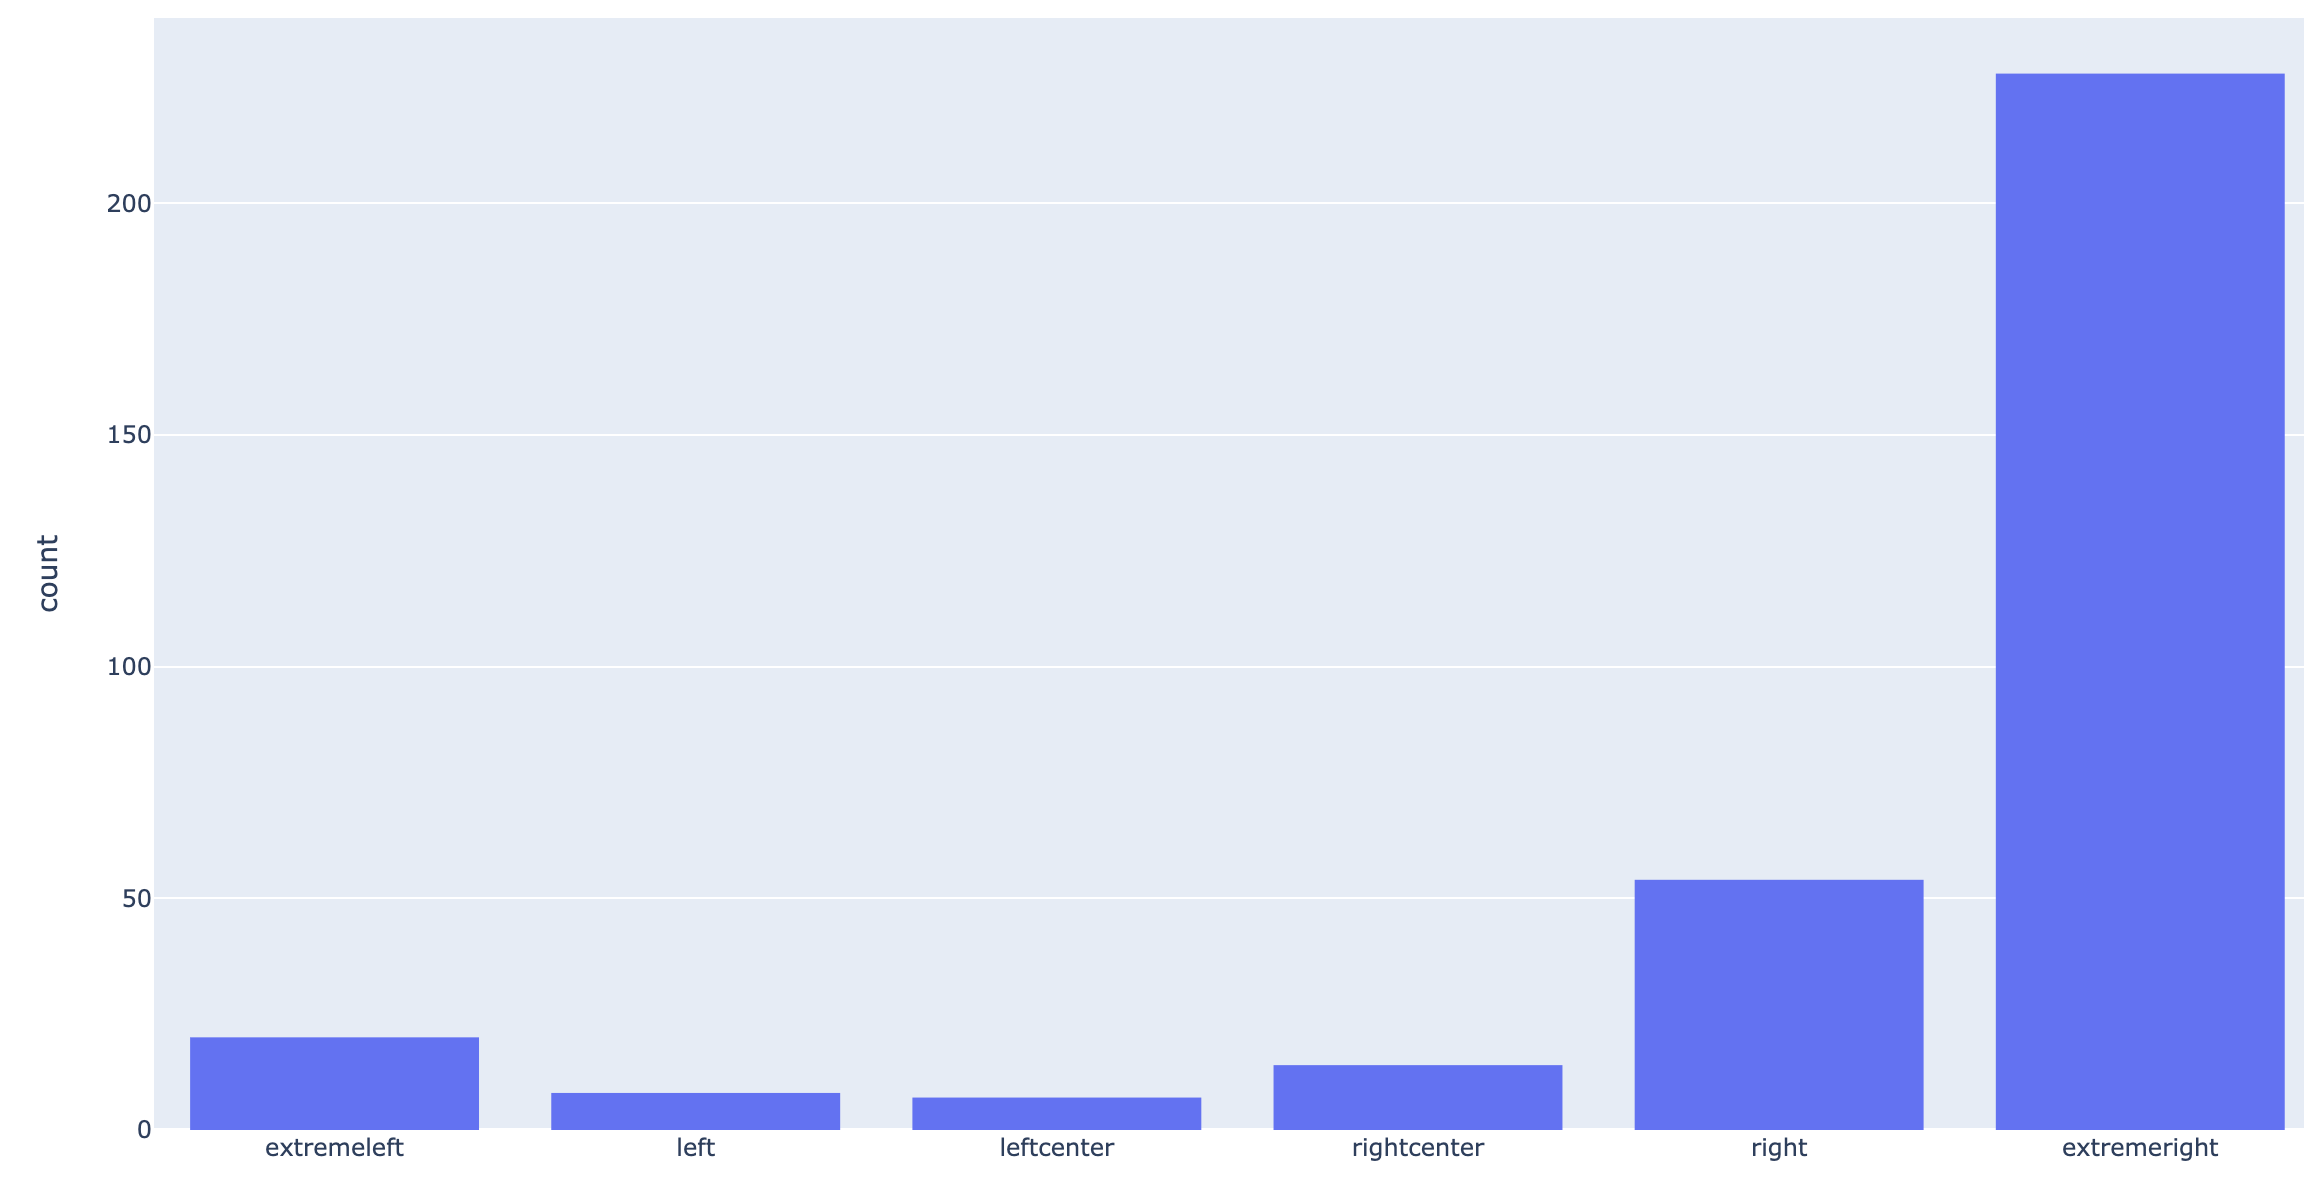
\includegraphics[width=\linewidth]{figures/leaning_questionable.png}
   \caption{The leaning of the propagandist sources from MBFC (TODO compare with effective training dataset, which is 100\% right)}
   \label{fig:mbfc_leaning}
\end{figure}

- Possible problems?
A possible problem of this approach that is not defended in the paper, is the choice of articles that have been annotated by experts. They have been selected from sources "propagandistic by Media Bias/Fact Check", in other words from the page \url{https://mediabiasfactcheck.com/fake-news/}. The propagandistic sources listed in this page, as Figure~\ref{fig:mbfc_leaning} shows, are mostly on the extreme-right side of the spectrum. Furthermore, the selection done by the authors (table 3 of that paper) results in all the sources of the articles to lean on the right.
So the resulting model is \textbf{being trained on very propagandistic sources from the right only}. The model will not be able to see left-propaganda because it never saw it in the training phase.



\subsubsection{Populism and Propaganda by leaning}

This is the continuation of Section~\ref{ssec:lp_techniques_populism_vs_propaganda} from the previous chapter. Now that we introduced the leaning and the problem of unbalance, we are going to break down the analysis with respect to the political leaning of the speeches.
% Dataset found: populism in political speeches %https://dataverse.harvard.edu/dataset.xhtml?persistentId=doi:10.7910/DVN/LFTQEZ&version=2.0 
% Each annotator (4 for each speech) gave a score between 0 (non-populistic) to 2 (very populistic)
% 4961 rows 
% 1240 deduped (352 left, 256 center, 469 right, 652 NA)
% Languages: 265 en (304 es, 148 pt, …),
% Leaning of the english ones: (36 left, 37 center, 84 right, 106 NA)

These 265 speeches all have a leaning classification (we will see more about leanings in the next chapter): 36 left, 37 center, 84 right, 106 NA. We use this information in order to check whether the results that we get are general across the political spectrum.

RESULTS

L/R evaluation:
Assumption: propaganda correlates to populism similarly in L/C/R
Result total: 0.225 Left, 0.005 Center, 0.374 Right → Why? Is it a matter of quantity of populism/propaganda?
Populism average:  [0.1259, 0.0729, 0.2712]
Propaganda average: [0.0165, 0.0271, 0.0432]
Ratio: [0.1317, 0.3717, 0.1593] → populism over propaganda ratio is a bit bigger on right (21\% more), but the correlation Right is bigger than left of 66\%. So it is less likely that this is just a matter of quantity. On the Right, propaganda and populism are strongly linked

Findings

Propaganda and populism are correlated, but not too strongly. In the Right more. This is one point supporting the hypothesis that propaganda detection works better in the Right than in the Left. → unbalanced detection caused by unbalanced data


\section{Discussions}
\label{sec:ps_discussions}

what was achieved, findings by RQ:

\begin{itemize}
    \item How does propaganda vary across the political spectrum? Less in the centre. More in the extremes. This was expected. Right seems to be more propagandistic, especially with some techniques (slogans, ...)
    \item Can we predict the political leaning of a news article by observing the propaganda it uses? Very difficult task. We see minimal effects
    \item Is Propaganda Detection balanced? Or is there some imbalance in the datasets used in the literature? Quite unbalanced datasets. Not clear what the effect of this imbalance is.
\end{itemize}

limitations

\section{Next}
\label{sec:ps_next}

Propaganda features are not enough to recognise leaning, and propaganda seems to be spread around in almost all leanings. We need to find whether, by including another dimension, we can differentiate better. 
Does it depend on the topics of the articles?

Need to break down by topic and see whether for some of them, propaganda of one leaning is very different from the one of the others.